%%%%%%%%%%%%%%%%%%%%%%%%%%%%%%%%%%%%%%%%%%%%%%%%%%%%%%%%%%%%%%%%%%%%%%%%%%%%%%%%
%2345678901234567890123456789012345678901234567890123456789012345678901234567890
%        1         2         3         4         5         6         7         8

\documentclass[letterpaper, 10 pt, conference]{ieeeconf}  % Comment this line out
                                                          % if you need a4paper
%\documentclass[a4paper, 10pt, conference]{ieeeconf}      % Use this line for a4
                                                          % paper
\usepackage{algorithm}
\usepackage{algorithmic}
\usepackage{booktabs}
\usepackage{graphicx}
\IEEEoverridecommandlockouts                              % This command is only
                                                          % needed if you want to
                                                          % use the \thanks command
\overrideIEEEmargins
% See the \addtolength command later in the file to balance the column lengths
% on the last page of the document



% The following packages can be found on http:\\www.ctan.org
%\usepackage{graphics} % for pdf, bitmapped graphics files
%\usepackage{epsfig} % for postscript graphics files
%\usepackage{mathptmx} % assumes new font selection scheme installed
%\usepackage{times} % assumes new font selection scheme installed
%\usepackage{amsmath} % assumes amsmath package installed
%\usepackage{amssymb}  % assumes amsmath package installed

\title{\LARGE \bf
DH2323 Computer Graphics and Interaction 
\linebreak GPU Raytracing with KD-trees
\linebreak Project Report
}


\author{Forrest Timour and Pooria Ghavamian} % <-this % stops a space





\begin{document}



\maketitle
\thispagestyle{empty}
\pagestyle{empty}


%%%%%%%%%%%%%%%%%%%%%%%%%%%%%%%%%%%%%%%%%%%%%%%%%%%%%%%%%%%%%%%%%%%%%%%%%%%%%%%%
\begin{abstract}


This paper provides a holistic overview of raytracing and its some of its optimization strategies. The role of acceleration structures is studied, and one such structure that takes advantage of spatial subdivision is implemented on a basic raytracer. Furthermore, the computational independence of rays is utilized in the implementation of a parallelized OpenCL-based GPU raytracer. Finally, the acceleration structure deployed earlier on a basic CPU based raytracer is integrated into the new GPU raytracer for maximum algorithmic optimization. Scenes with varying triangle counts are tested, and a staggering 99.9 \% drop in render time for some of our larger models is demonstrated. 


\end{abstract}

\textit{\textbf{keywords:} GPU Raytracing, OpenCL, KD-trees } 

%%%%%%%%%%%%%%%%%%%%%%%%%%%%%%%%%%%%%%%%%%%%%%%%%%%%%%%%%%%%%%%%%%%%%%%%%%%%%%%%
\section{INTRODUCTION}

Raytracing is a rendering technique that is becoming increasingly popular with the emergence of powerful hardware and algorithms that allow very expensive near-photorealistic visual imagery to be produced in real time. A large amount of research and effort has been funneled down the path of real time raytracing and companies like Nvidia have recently announced products like \textit{NVIDIA RTX™ Technology} that show great promise. In this project, we will be making use of spatial raytracing acceleration structures, to optimize intersection finding by subdividing the bounding box into smaller boxes recursively, effectively partitioning the large triangle set into much smaller sets that can be skipped during intersection finding by selective branch pruning for nodes whose bounding boxes do not intersect with a ray. Moreover, we will take advantage of the abundant parallelization opportunities offered to us by the raytracing algorithm by implementing it on the GPU.


\section{Implementation}
This section focuses more on the overall approach to the implementation and the rationale behind it. A detailed step-by-step documentation of our implementation is being written and will be provided in the project blog \cite{c2}.
\subsection{Basic Raytracer with Spatial Subdivision}
 Before moving into GPU programming, a basic Whitted Raytracer was implemented based on the recursive design introduced in "An Improved Illumination Model for Shaded Display"\cite{c1} . The core mechanism of the raytracer is straightforward. Our basic raytracer is comprised mostly of two parts:
 
\begin{itemize}
\item Shading
\item Intersection calculation
\end{itemize}
 
Given a scene with \textit{N} primitives, a basic raytracer will do intersection tests for each primitive with a total time complexity of \textit{O(N)}. Shading is also done in \textit{O(N)} time, checking all \textit{N} primitives again in order to account for the blocked path of light. Therefore, execution profiling (identifying hotspots in a program) suggests that a reasonable starting point for optimization is the intersection test between a ray and the scene.

The total time spent in an application can be broken down as such\cite{c3}:

\[\mathtt{total\_time} = \sum_{i=0} ^{\#\mathtt{tasks}}\mathtt{time}_i\]
\[\mathtt{time}_i= \frac{\mathtt{work}_i}{\mathtt{rate\_of\_work}_i}\]

According to this formula we can either carry out a low-level optimization of the time it takes to do task \textit{\textbf{i}}, or reduce the number of times task \textit{\textbf{i}} itself is carried out. Using acceleration structures we can cut the number of unnecessary intersections tests without significantly altering the execution of our naive raytracer. Acceleration structures can be implemented using \textit{object hierarchies} or \textit{spatial subdivision}. In this project we opted for spatial subdivision using KD-trees and bounding boxes.

Initially, we start with a bounding box that encompasses the entire scene. This box is recursively subdivided until a terminating condition is met. The splits can be done in a way that optimizes the structure of the KD-tree. One such method, called the \textit{Surface Area Heuristic (SAH)}, involves splitting based on surface area of primitives. The basic idea is that the probability of a ray hitting a voxel is correlated to its respective surface area. For the purposes of this project, however, we split at the midpoints of longest dimensions. After building the KD-tree, we can recursively traverse it and find the intended intersection. A form of such traversal is shown in Algorithm 1.  

\begin{algorithm}[H]
\caption{KD-tree Traversal}
\begin{algorithmic}

\IF{leaf node reached}
    \STATE intersect with triangles
    \IF{intersection is true}
    \STATE pick closest intersection and return 
    \ENDIF
\ELSE
    \STATE intersect with AABB split 
    \IF {intersection with closer box}
        \STATE recurse on closer box
    \ENDIF
    \IF {no intersection yet AND intersection with farther box}
        \STATE recurse on farther box
    \ENDIF
    \STATE return intersection if found, or none
\ENDIF
\end{algorithmic}
\end{algorithm}

\subsection{Parallelization using GPU}

Acceleration structures can greatly improve the performance of our raytracer. However, more improvement can be done by noting the fact that each ray is independent of all the others, and therefore a parallelized solution can significantly increase performance. This is done by running smaller programs, called Kernels, on all available GPU compute units using OpenCL. These compute units (or CUDA cores, Stream Processors, etc.) typically have a lower clock speed than CPU cores, but give an overall performance boost by sheer numbers, hardware-implemented functions, and optimized compilers. The theoretical compute time is given by:
\[T_P=S\times\mathtt{work}(n)+\frac{(1-S)\times\mathtt{work}(n)}{P}\]
where $S$ is the inherently sequential part of the work (for example loading the scene into memory) and $P$ is the number of parallelizable pieces (compute units available). This gives us ideally a perfect linear speedup of
\[\frac{T}{T_P}\approx\frac{1}{S+\frac{1-S}{SP}}\]
(modulo time for scheduling and overhead of splitting work).

\subsection{KD-Trees on the GPU}
One of the inherent limitations of GPU programming with OpenCL is the lack of recursion, making it difficult to traverse inherently recursive data structures like KD-Trees. We solved this hurdle by unrolling the tree into a one-dimensional array, using absolute indices for child nodes rather than pointers. This comes at the expense of some low-level optimization that could otherwise be done, but the benefits far outweigh the drawbacks in this regard. Traversal was done iteratively with hard-coded pseudo-stack array to keep track of nodes that still had to be checked.

\section{results}
To have a quantitative gauge for the performance of the raytracer, tests were carried out. The experimentations were designed to first measure the optimal depth of the KD-tree, and then quantify the improvement of our raytracer at different levels of its implementation. These tests were done on a low/mid-tier laptop using an Intel i5 CPU and Intel Integrated Graphics (with a total of 24 compute units), far from the high-power computational tools available today. The following are results for the calculation of the ideal depth of the KD-Tree cutoff.


\begin{table}[H]

\begin{tabular}{@{}llll@{}}
\toprule
Depth & Cornell Box(ms) & Tiny Dragon (ms) & Medium Dragon(ms) \\ \midrule
1     & 42.0            & 2668.0           & 9944.0            \\
2     & 49.0            & 550.0            & 10217.0           \\
3     & 59.0            & 286.0            & 6200.0            \\
4     & 64.0            & 211.0            & 4236.0            \\
5     & 64.0            & 176.0            & 3306.0            \\
6     & 68.0            & 154.0            & 2668.0            \\
7     & 62.0            & 143.0            & 2245.0            \\
8     & 66.0            & 166.0            & 2208.0            \\
9     & 64.0            & 201.0            & 2448.0            \\
10    & 65.0            & 303.0            & 3081.0            \\
11    & 66.0            & 442.0            & 4504.0            \\
12    & 70.0            & 550.0            & 7201.0            \\
13    & 72.0            & 647.0            & 9253.0            \\
14    & 67.0            & 706.0            & 10706.0           \\
15    & 64.0            & 735.0            & 12923.0           \\ \bottomrule
\end{tabular}\\

table 1: KD cutoff results
\end{table}

The table produces the following chart:

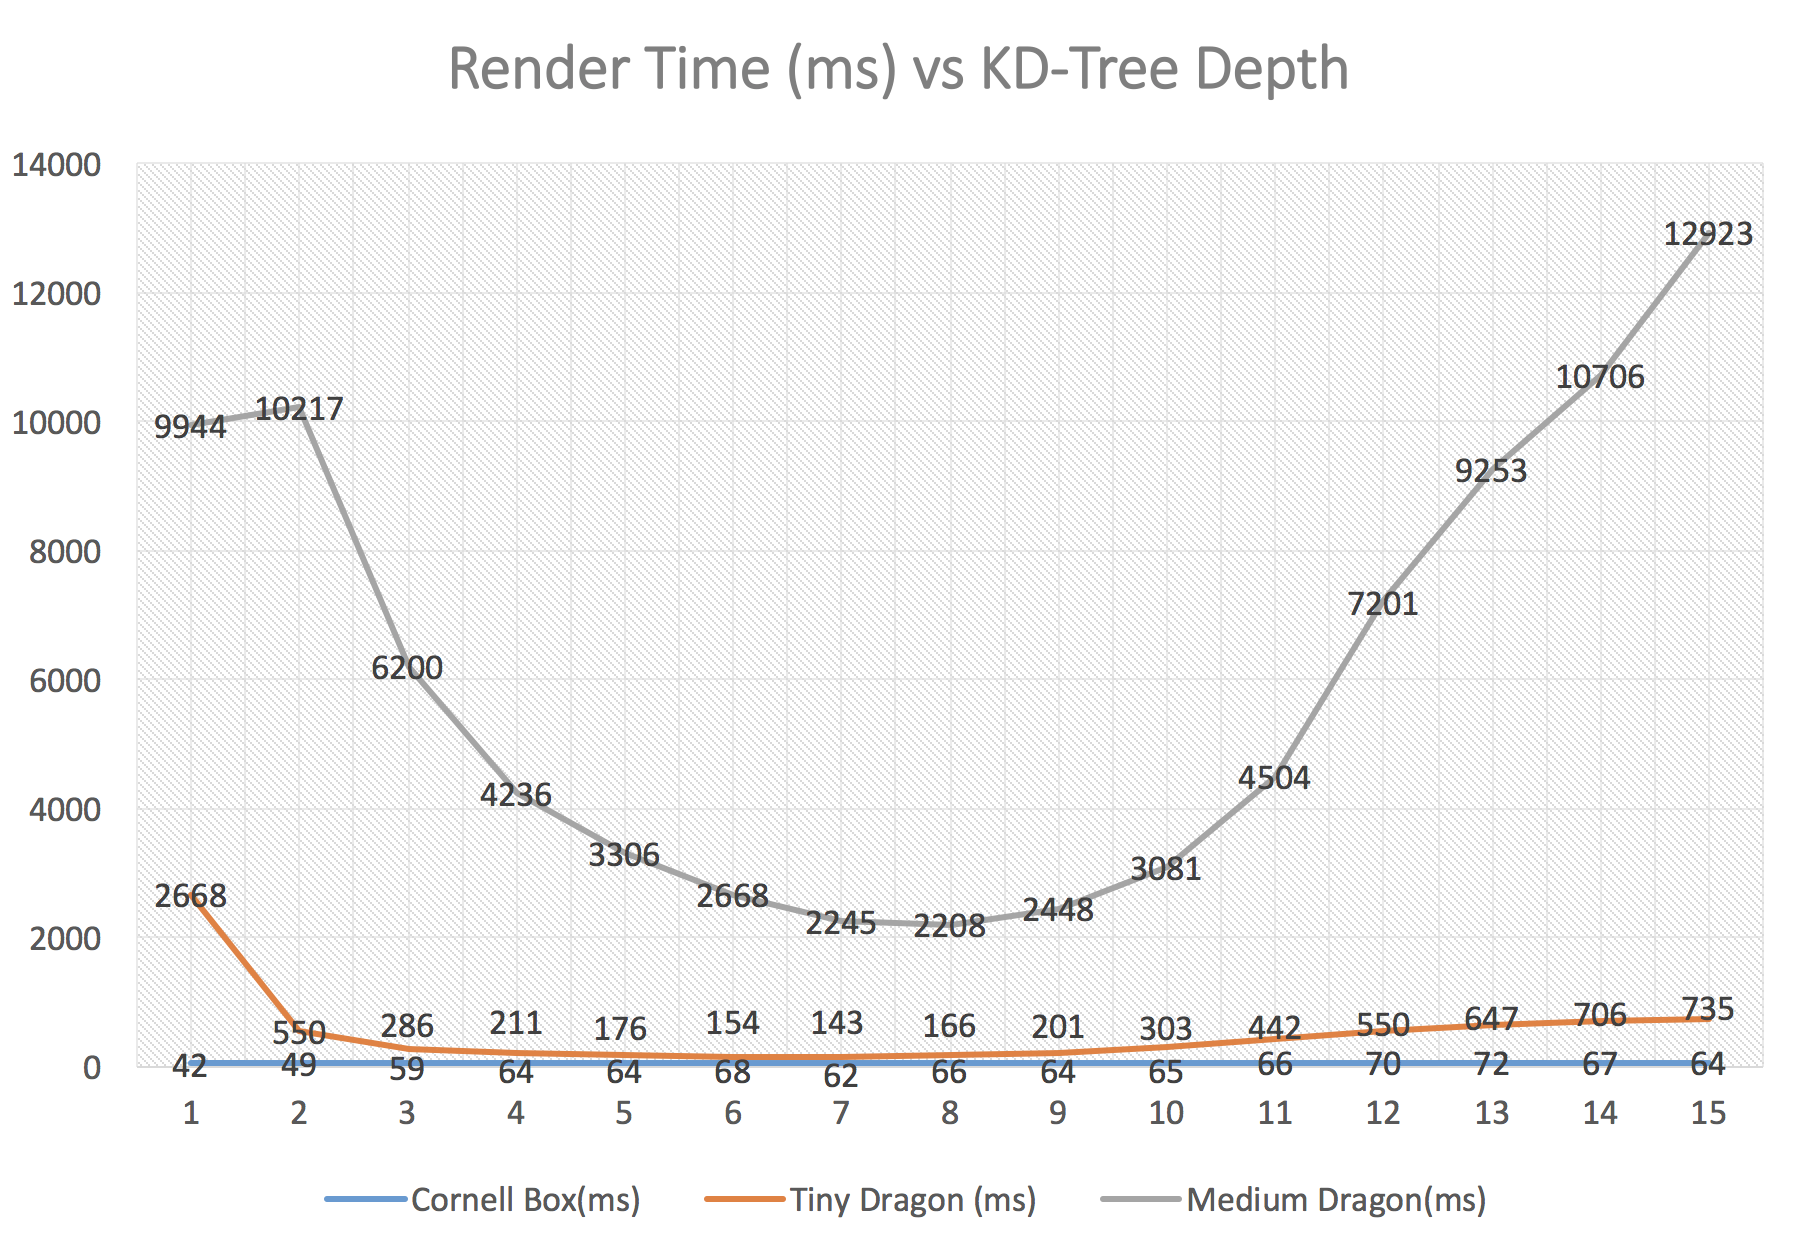
\includegraphics[width=.95\columnwidth]{chart_1.png} 
{\small\textit{figure 1: results of KD-tree depth comparison}}

As it can be seen, the ideal tree depth is about 7 or 8 for larger models before the overhead of traversal and redundant box-overlapping triangles becomes too much. Naturally, very small models start to suffer at lower depths than large models, where the ideal depth is expected to grow logarithmically. Finally, trials were done to measure how the render time reacts to different strategies at different triangle counts (see table 2).

\begin{table*}[t]
\centering
\begin{tabular}{@{}llllll@{}}
\toprule
Raytracer     & Cornell Box(ms) & Tiny Dragon (ms) & Small Dragon (ms) & Medium Dragon(ms) & Large Dragon(ms) \\ \midrule
Naive         & 3979.0          & 674659.0         & 2832750.0         & -----         &                  ----\\
KD-tree       & 9728.0          & 25405.0          & 104268.0          & 371202.0          & 1115250.0        \\
GPU           & 44.0            & 2157.0           & 12878.0           & 10411.0           & 11375.0          \\
GPU + KD-tree & 68.0            & 152.0            & 509.0             & 2236.0            & 10234.0          \\ \bottomrule
\end{tabular}\\

table 2: Render time results
\end{table*}

\section{Discussion}
Here we will briefly talk about the design decisions we made during the iterative process of improving our ray tracer(s). One such decision was to re-use the same code as much as possible, in the interest of avoiding confusion between different parts of the project. For example, in the final iteration of the project, construction of the KD-Tree \textit{array} was first done recursively, and then traversed again to be flattened. This makes the construction complexity $(n^2+n)$ with heuristic optimizations, which is still $\mathcal{O}(n^2)$ but with extra overhead. In such cases we deemed it unnecessary to optimize further.

We also chose the KD-Tree splitting heuristic of spatial median partitioning rather than primitive-dependent partitioning, with the naïve implicit assumption that the distribution of primitives was uniform throughout the scene. This has the possibility to lead to unbalanced binary KD-Trees in non-uniform models, which we did not test comprehensively.

We did not implement reflection and refraction, and limited the recursion depth to only two, to allow shadows. The purposes of our project were algorithmic exploration and rendering speed rather than photo-realism, so we deemed this okay as well.
\section{CONCLUSIONS}
Results of the optimal KD-Tree depth were lower than we expected, likely because of the number of triangles overlapping multiple sub-boxes. The results of the naïve raytracer were expectedly horrendous on the larger models, so we ended up giving up on collecting data for the largest two scenes. Both the KD-Tree raytracer and the GPU raytracer improved the performance immensely, but we were surprised that the GPU speedup was so much higher than that of the KD-Tree. The KD-Tree raytracer is expected to have better asymptotic performance, as the speedup was done algorithmically rather than linearly.

Overall, our GPU + KD-Tree raytracer performed the best, and we were very satisfied with the results we saw. We are unable to explain why the rendering time for the medium and large dragons with the GPU raytracer are so similar, but they were tested multiple times in order to be verified.

\addtolength{\textheight}{-12cm}   % This command serves to balance the column lengths
                                  % on the last page of the document manually. It shortens
                                  % the textheight of the last page by a suitable amount.
                                  % This command does not take effect until the next page
                                  % so it should come on the page before the last. Make
                                  % sure that you do not shorten the textheight too much.

%%%%%%%%%%%%%%%%%%%%%%%%%%%%%%%%%%%%%%%%%%%%%%%%%%%%%%%%%%%%%%%%%%%%%%%%%%%%%%%%

\section*{Future work}
We did not have as much time as we did ambition, so here are some of things we didn't get to this time (but would like to do in the future).
\begin{itemize}
\item Optimal KD-Tree construction in $\mathcal{O}(n\log{n})$
\item Implementing a BVH to compare with the KD-Tree
\item Support for other graphical primitives, such as spheres
\item Exploring precalculation for intersection finding
\item More optimization, at the expense of code duplication between versions
\item Comparison of OpenCL and CUDA
\item Comparing results on multiple setups
\item Code profiling and optimization where possible
\end{itemize}

%%%%%%%%%%%%%%%%%%%%%%%%%%%%%%%%%%%%%%%%%%%%%%%%%%%%%%%%%%%%%%%%%%%%%%%%%%%%%%%%

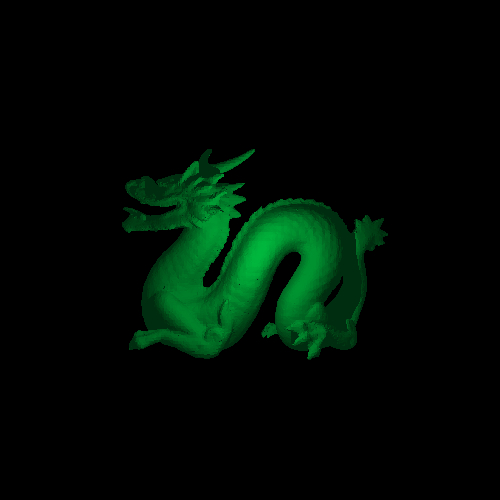
\includegraphics[width=.95\columnwidth]{dragon.jpg} 
{\small\textit{figure 2: rendering of the dragon at 500x500 resolution}}

\begin{thebibliography}{99}

\bibitem{c1} Whitted, T. (1980). An improved illumination model for shaded display. Communications Of The ACM, 23(6), 343-349. doi: 10.1145/358876.358882

\bibitem{c2} Timour, F. and Ghavamian, P. (2018). Tumblr. [online] How Do Ray Do it?. Available at: https://howdoraydoit.tumblr.com/ [Accessed 1 Aug. 2018].
\bibitem{c3}Azillionmonkeys.com. (2018). Programming Optimization: Techniques, examples and discussion. [online] Available at: http://www.azillionmonkeys.com/qed/optimize.html [Accessed 3 Aug. 2018].




\end{thebibliography}




\end{document}
